% -%-%-%-%-%-%-%-%-%-%-%-%-%-%-%-%-%-%-%-%-%-%-%-%-%
% FLE % 
% Data:28/11/2011                                 %
% Paris,France                                    % 
% Groupe:                                         %
% - Tiago Chedraoui Silva                   % 
% - Angie Anazgo la Rosa %
% -%-%-%-%-%-%-%-%-%-%-%-%-%-%-%-%-%-%-%-%-%-%-%-%-%

\documentclass[a4paper,11pt]{article}

\usepackage[francais,listings,algo]{tcs}

% Cover %
\def \ttprofname{Roland BADEAU} % teachers name
\def \ttabrv{MDI224} % abbreviation of names class
\def \ttabrvxt{} % period
\def \mytitle{Interpolation par splines cubiques} % Big title
\def \mysubtitle{ Travaux Pratique 1 - Deuxième semestre de 2011} % subtitle
\def \ttauthi{} % author's name
\def \ttxti{} % Extra text right side of name
\def \ttauthii{Tiago Chedraoui Silva} % author's name
\def \ttxtii{Casier: 214 } % Extra text right side of name
\def \ttdate{Décembre 15, 2011} % date

\begin{document}
\titleTMB 
\newpage
\tableofcontents
\newpage

\section{Résolution du système linéaire}

\subsection{Méthode de Jacobi}
\subsubsection{Implémentation}

\begin{multicols}{2}
  \lstinputlisting[title=\textbf{Méthode de Jacobi}]{../jacobi.m}
\end{multicols}

\newpage
\subsubsection{Convergence}
\begin{figure}[h!]
  \begin{centering}
    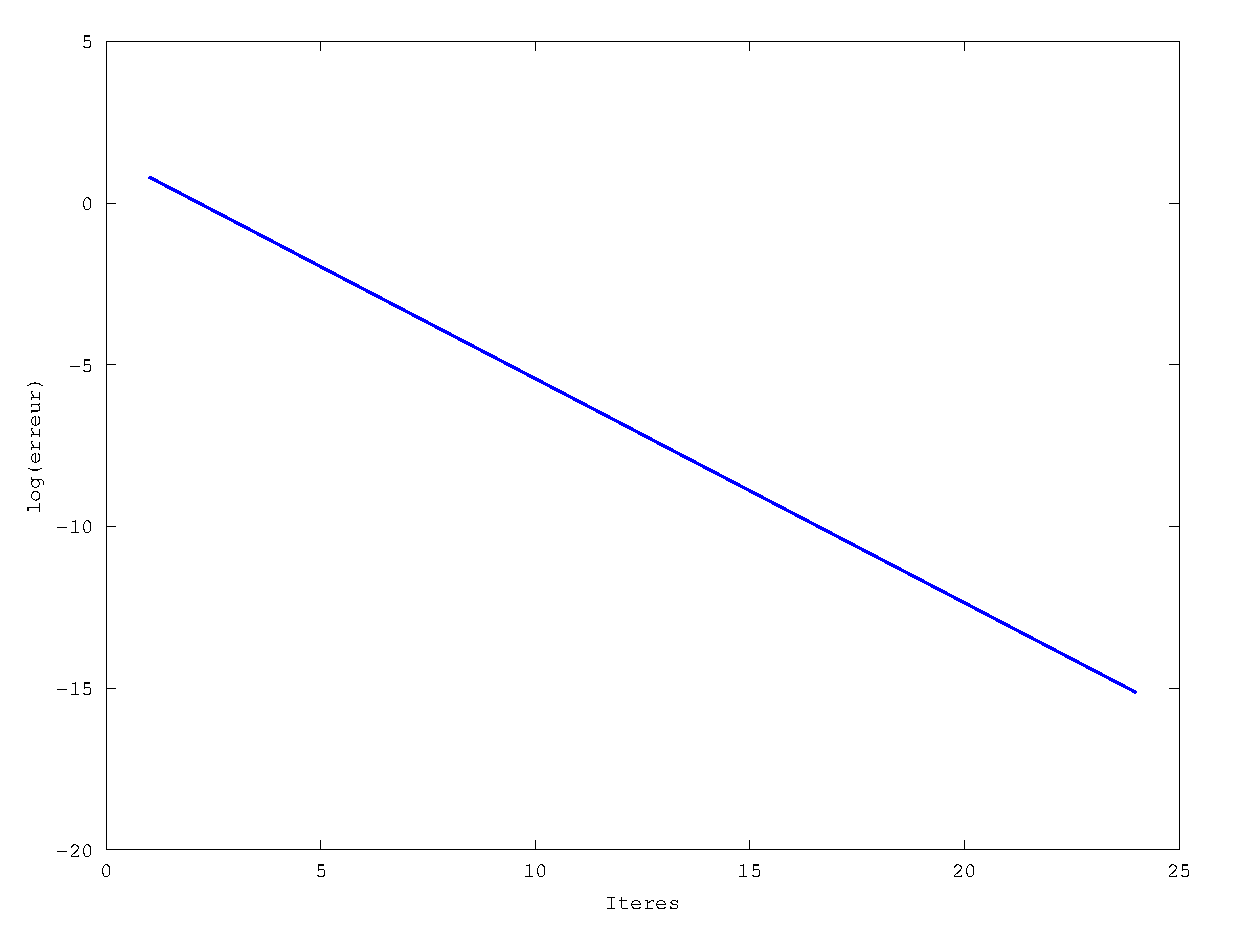
\includegraphics[scale=0.5]{../jacobi_graph}
    \label{rspro2}
    \par\end{centering}
  \caption{Convergence de la méthode de Jacobi}
  \label{fig:jacobi-conv}
\end{figure}

En utilisant la fonction polyfit, nous avons trouvé le polynome: 
$p(x)= -0.693147 x + 1.903331 $


\subsection{Méthode de relaxation}
\subsubsection{Implémentation}
\begin{multicols}{2}
  \lstinputlisting[title=\textbf{Méthode de Jacobi}]{../relax.m}
\end{multicols}

\subsubsection{Convergence}
\begin{figure}[h!]
  \begin{centering}
    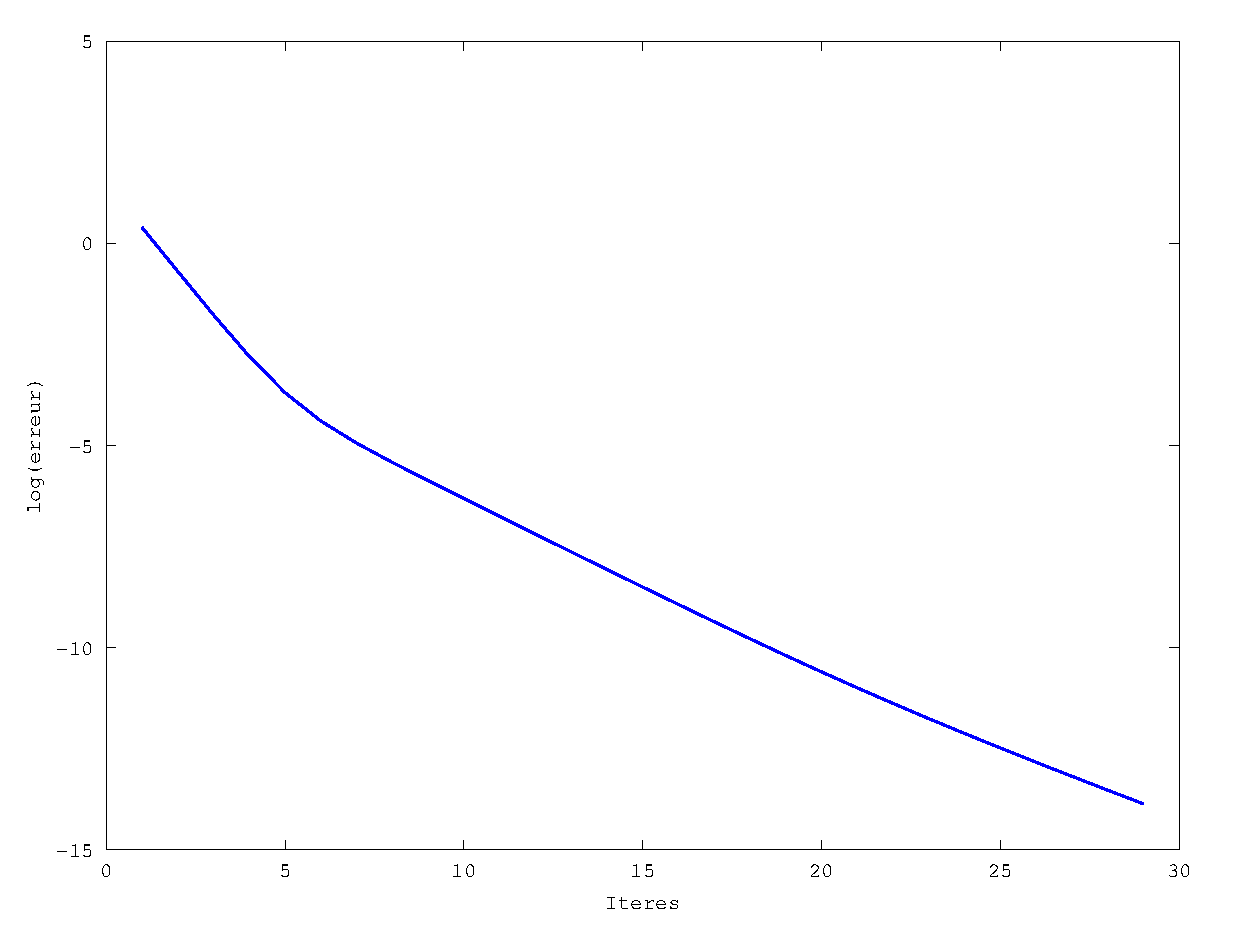
\includegraphics[scale=0.5]{../relaxation_graph}
    \label{rspro2}
    \par\end{centering}
  \caption{Convergence de la méthode de Relaxation pour w=1.0}
  \label{fig:jacobi-conv}
\end{figure}


\begin{figure}[h!]
  \begin{centering}
    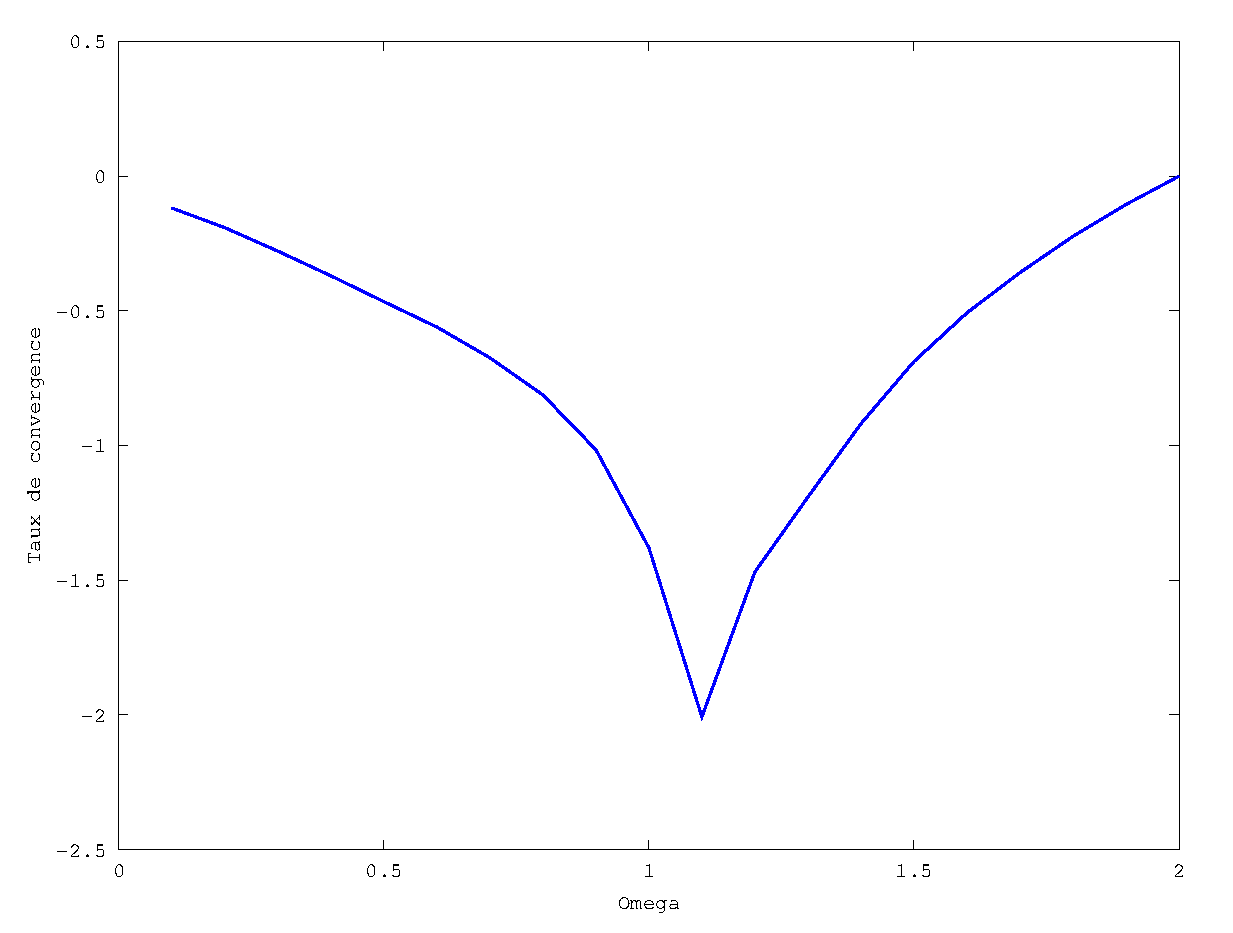
\includegraphics[scale=0.5]{../relaxation_conv}
    \label{rspro2}
    \par\end{centering}
  \caption{Taux de convergence en fonction du paramètre de relaxation w}
  \label{fig:jacobi-conv}
\end{figure}

\begin{equation}
  \omega = \frac{2}{1+\sqrt{1- \rho(J)^2}}
\end{equation}

\begin{equation}
  \frac{d\omega}{d\rho} =\frac{2\,\rho}{\sqrt{1-{\rho}^{2}}\,{\left( \sqrt{1-{\rho}^{2}}+1\right) }^{2}}
\end{equation}

Pour le valeur  minimum ou maximum la dérivée doit être  0, donc $\rho(J)=0$, en
utilisant la équation 1 on a $\omega=1$;

\newpage
\subsection{Méthode de Cholesky}
\subsubsection{Implémentation}

La fonction suivante était fournit par le problème. 
\begin{multicols}{2}
  \lstinputlisting[title=\textbf{Méthode de Jacobi}]{../cholesky.m}
\end{multicols}

Pour le même exemple précedent, on a trouve:

\begin{table}[h!]
  \begin{center}
    \begin{tabular}{|c|c|}
      \hline 
      p & x \\
      \hline 
      \hline 
      4 & [ 1.00000;1.00000;1.00000;1.00000;1.00000]\\
      3 & [ 1.00000;1.00000;1.00000;1.00000;1.00000]\\
      2 & [ 1.00000;1.00000;1.00000;1.00000;1.00000]\\
      1 & [ 1.00000;1.00000;1.00000;1.00000;1.00000]\\
      \hline 
    \end{tabular}
  \end{center}
  \caption{Vérification function Cholesky}
\end{table}

\subsubsection{Complexité}

\begin{table}[h!]
  \begin{center}
    \begin{tabular}{|c|c|c|c|c|c|c|}
      \hline 
      N & 50 & 100 & 150 & 200 & 250 & 300 \\
      \hline 
      \hline 
      Cholesky $(p=1)$ & 0.011554       &  0.023093 & 0.036068
      & 0.047571 & 0.061026 & 0.074059 \\
      Jacobi &  0.0013079
      &   0.0024460
      &  0.0026030
      &  0.0034651
      &  0.0058240
      & 0.012277\\
      Relaxation $(w = 1.1)$
      & 0.0011869 & 0.0017610
      &0.0029701 & 0.0057600
      & 0.0074950 & 0.014658\\
      \hline 
    \end{tabular}
  \end{center}
  \caption{Comparaison de temps entre les trois méthodes pour un système tridiagonal}
\end{table}

En  général le  méthode Jacobi est la  méthode plus  rapide pour  un
système tridiagonal.

\section{Application}
\subsection{Calcul d'une spline d'interpolation}
\subsection{Évaluation d'une fonction spline cubique}
\subsection{Application}

\end{document}

